\section{Linear Maps}
\begin{center}
    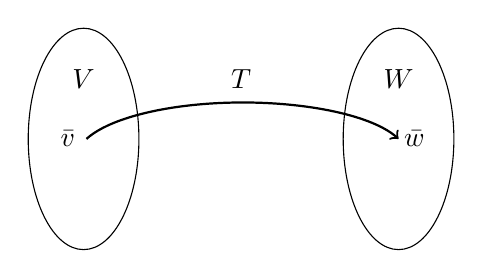
\begin{tikzpicture}
        \draw (2,0) ellipse (20pt and 40pt);
        \draw[] (-2,0) ellipse (20pt and 40pt);
        \draw[<-, thick] (2,0) arc (20:160: 60pt and 20pt);
        \draw (0,1)  node[anchor = north] {$T$};
        \draw (2,1)  node[anchor = north] {$W$}; 
        \draw (-2,1) node[anchor = north] {$V$};
        \draw (-2.2,0) node {$\bar v$};
        \draw (2.2,0) node {$\bar w$};
    \end{tikzpicture}
\end{center}

Suppose $V$ and $W$ are two linear spaces over $\b F$. $T$ is a function with domain $V$ and codomain $W$. $T$ is called linear iff 
\begin{enumerate}
    \item $T(\bar v_1 + \bar v_2) = T(\bar v_1) + T(\bar v_2)$
    \item $T(\lambda \bar v) = \lambda \cdot T(\bar v)$
\end{enumerate}
$\forall \bar{v}_1, \bar{v}_2 \in V$ and $\forall \bar{v} \in V, \forall \lambda v \in \b F$.
\begin{example}
    Let $V = \b R^3, W = \b R^4$. Define $T$ as $(x_1, x_2, x_3) \mapsto (x_1,0,0,0)$
\end{example}
\begin{example}
    $T: \c P(x) \to \c P(x)$, where $\displaystyle f(x) \mapsto \int_{10}^x f(x) \ dx$ is a linear map.
\end{example}
\begin{definition}
    $\c L\{V, W\}$ denotes the set of all linear maps from $V$ to $W$. Note that $\c L\{V, W\}$ with $+$ and $\cdot$ becomes a vector space over $\b F$. This requires the additions of functions and multiplications of linear maps by scalars (from $\b F$). Given $T_1, T_2 \in \c L(V,W)$ we define addition as $(T_1 + T_2)(\bar v) := T_1(\bar v) + T_2(\bar v)$, multiplication as $(\lambda T)(\bar v) : = \lambda \cdot T(\bar v)$. 
\end{definition}
\begin{theorem}
    In finite vector space $V,W$, let $\li{\bar v}n$ be a basis for $V$, let $\li{\bar w}m$ be any vectors in $W$. Then there exist a unique linear map $T \in \c L \lb V, W \rb$ such that $T(\bar v_j) = \bar w_j \forall j$.
\end{theorem}
\begin{proof}
    Any vector in $V$ has a unique representation $\alpha_1 \bar v_1 + \alpha_2\bar v_2 + \cdots + \alpha_n \bar v_n = \bar v$.  \\ Define $T(\bar v):= \underbrace{\lincomb \alpha {T(\bar v)}n}_{\in W}$ This makes $T$ a linear map from $V$ to $W$. Indeed if $\lambda \in \b F$, then $T(\lambda \bar v) = T(\sum_{j = 1}^n \lambda \alpha_j \bar v_j) = \lambda \sum_{j = 1}^n \alpha_j \bar wj$. Suppose $\tilde T(\bar v_j) = \bar w_j$ for all $j$, then $T = \tilde T$ as a map function by linearity and basis.
\end{proof}
\begin{theorem}
    Let $\nul (T):= \lb \bar v \in  v : T(\bar v) = 0 \rb$. $\nul (T)$ is a subspace of $V$.
\end{theorem}
\begin{theorem}
    Let $\range (T):= \lb \bar w \in W : T(\bar v) = \bar w \rb$. $\range(T)$ is a subspace of $W$.
\end{theorem}
\begin{proof}
    The proof is trivial and is left as an exercise for the reader .
\end{proof}
\begin{example}
    Let $T: f \to f', V:= \c P(x), W:= \c P(x)$. $\nul(T) = \c P_0(x)$, $\range(T) = \c P_2(x)$. \\
    Let $T: f \to f'', V:= \c P(x), W:= \c P(x)$. $\nul(T) = \c P_1(x)$, $\range(T) = \c P_1(x)$.
\end{example}
\begin{example}
    Find a basis of $\c L (V,W)$ given bases $\lb \li {\bar v}m \rb$ and $\lb \li{\bar w}n \rb$ of $V$ and $W$. \\
    The basis consists of $m \times n$ vectors as follows: 
    \[T_{11} = T(\bar v_1) = \bar w_1, T(\bar v_2) = \bar 0, T(\bar v_3) = \bar 0, \ldots ,T(\bar v_m) = \bar 0\]
    \[T_{12} = T(\bar v_1) = \bar w_2, T(\bar v_2) = \bar 0, T(\bar v_3) = \bar 0, \ldots ,T(\bar v_m) = \bar 0\]
    \[ \cdots \]
    \[T_{mn} = T(\bar v_1) = \bar 0, T(\bar v_2) = \bar 0, T(\bar v_3) = \bar 0, \ldots ,T(\bar v_m) = \bar w_n\]
\end{example}
\begin{example}
    Let $\c U = \lb f : \b R \to \b R : f(x) = f(1-x) \ \forall x \rb$.
    \begin{enumerate}
        \item Show that $\c U$ is a subspace of $f: \b R \to \b R$. 
        \begin{proof}
            We can see that the zero function $f(x) = 0$ satisfies the requirement since $0 = 0$ for all  values of $x$. 
            
            Suppose $f(x), g(x) \in \c U$, then we compute \begin{align*}
                (f + g)(x) &= f(x) + g(x) \\
                           &= f(1 - x) + g(1 - x) \\
                           &= (f + g)(1 - x)
            \end{align*}
            Therefore we can see that $\c U$ is closed under addition.
            
            Suppose $f(x) \in \c U, \lambda \in \b R$, then we compute \begin{align*}
                (\lambda \cdot f)(x) &= \lambda \cdot f(x) \\
                                     &= \lambda \cdot f(1 - x) \\
                                     &= (\lambda \cdot f)(1 - x)
            \end{align*}
            Therefore we can see that $\c U$ is closed addition. 
            
            Hence $\c U$ is a vector space.
        \end{proof}
        \item Find a complement.
        \[ \c W  = \lb g : \b R \to \b R : g(x) = -g(1 - x) \ \forall x \rb\]
        \begin{proof}
            The proof for subspace is similar to part (i) and is omitted here. \\
            We now want to show that $\c U + \c W  = \mathbb{R}^{\mathbb{R}}$. We can see that for $f(x) \in \mathbb{R}^{\mathbb{R}}$, we can rewrite $f(x)$ as
            \[ f(x) = \frac{f(x) + f(1 - x)}{2} + \frac{f(x) - f(1 - x)}{2}\]
            Clearly $\displaystyle \frac{f(x) + f(1 -x)}{2} \in \c U$ and $\displaystyle \frac{f(x) - f(1 - x)}{2} \in \c W$. For uniqueness, suppose that a nonzero $h(x) \in \c U \cap \c W$, therefore $h(x) = h(1 - x) = -h(1 - x)$, and the only solution is $f(x) = 0$, a contradiction, therefore $\c U \cap \c W = \lb 0 \rb$. Hence $\boxed{{\b R^{\b{R}}} = \c U \oplus \c W}$
        \end{proof}
    \end{enumerate}
\end{example}

